\section{Results}
\label{sec:results}

\subsection{Centrality Analysis — Higgs Twitter}

Figure~\ref{fig:mention_centrality} (Section~\ref{sec:model}) shows the
top-15 nodes for the Mention network.
A consistent pattern emerges across all three Higgs networks: a single
dominant hub (node \texttt{88}) captures the highest in-degree and
eigenvector centrality, while a structurally distinct bridge node
(node \texttt{64911} in Retweet, \texttt{13808} in Reply) leads in
betweenness centrality.
This \textit{hub--bridge duality} suggests that the most-mentioned accounts
are not necessarily the primary conduits through which information flows
between communities.

Figure~\ref{fig:retweet_centrality} provides the equivalent four-panel view
for the Retweet network, which is the largest and most influential propagation
channel during the Higgs boson event.

\begin{figure*}[!t]
    \centering
    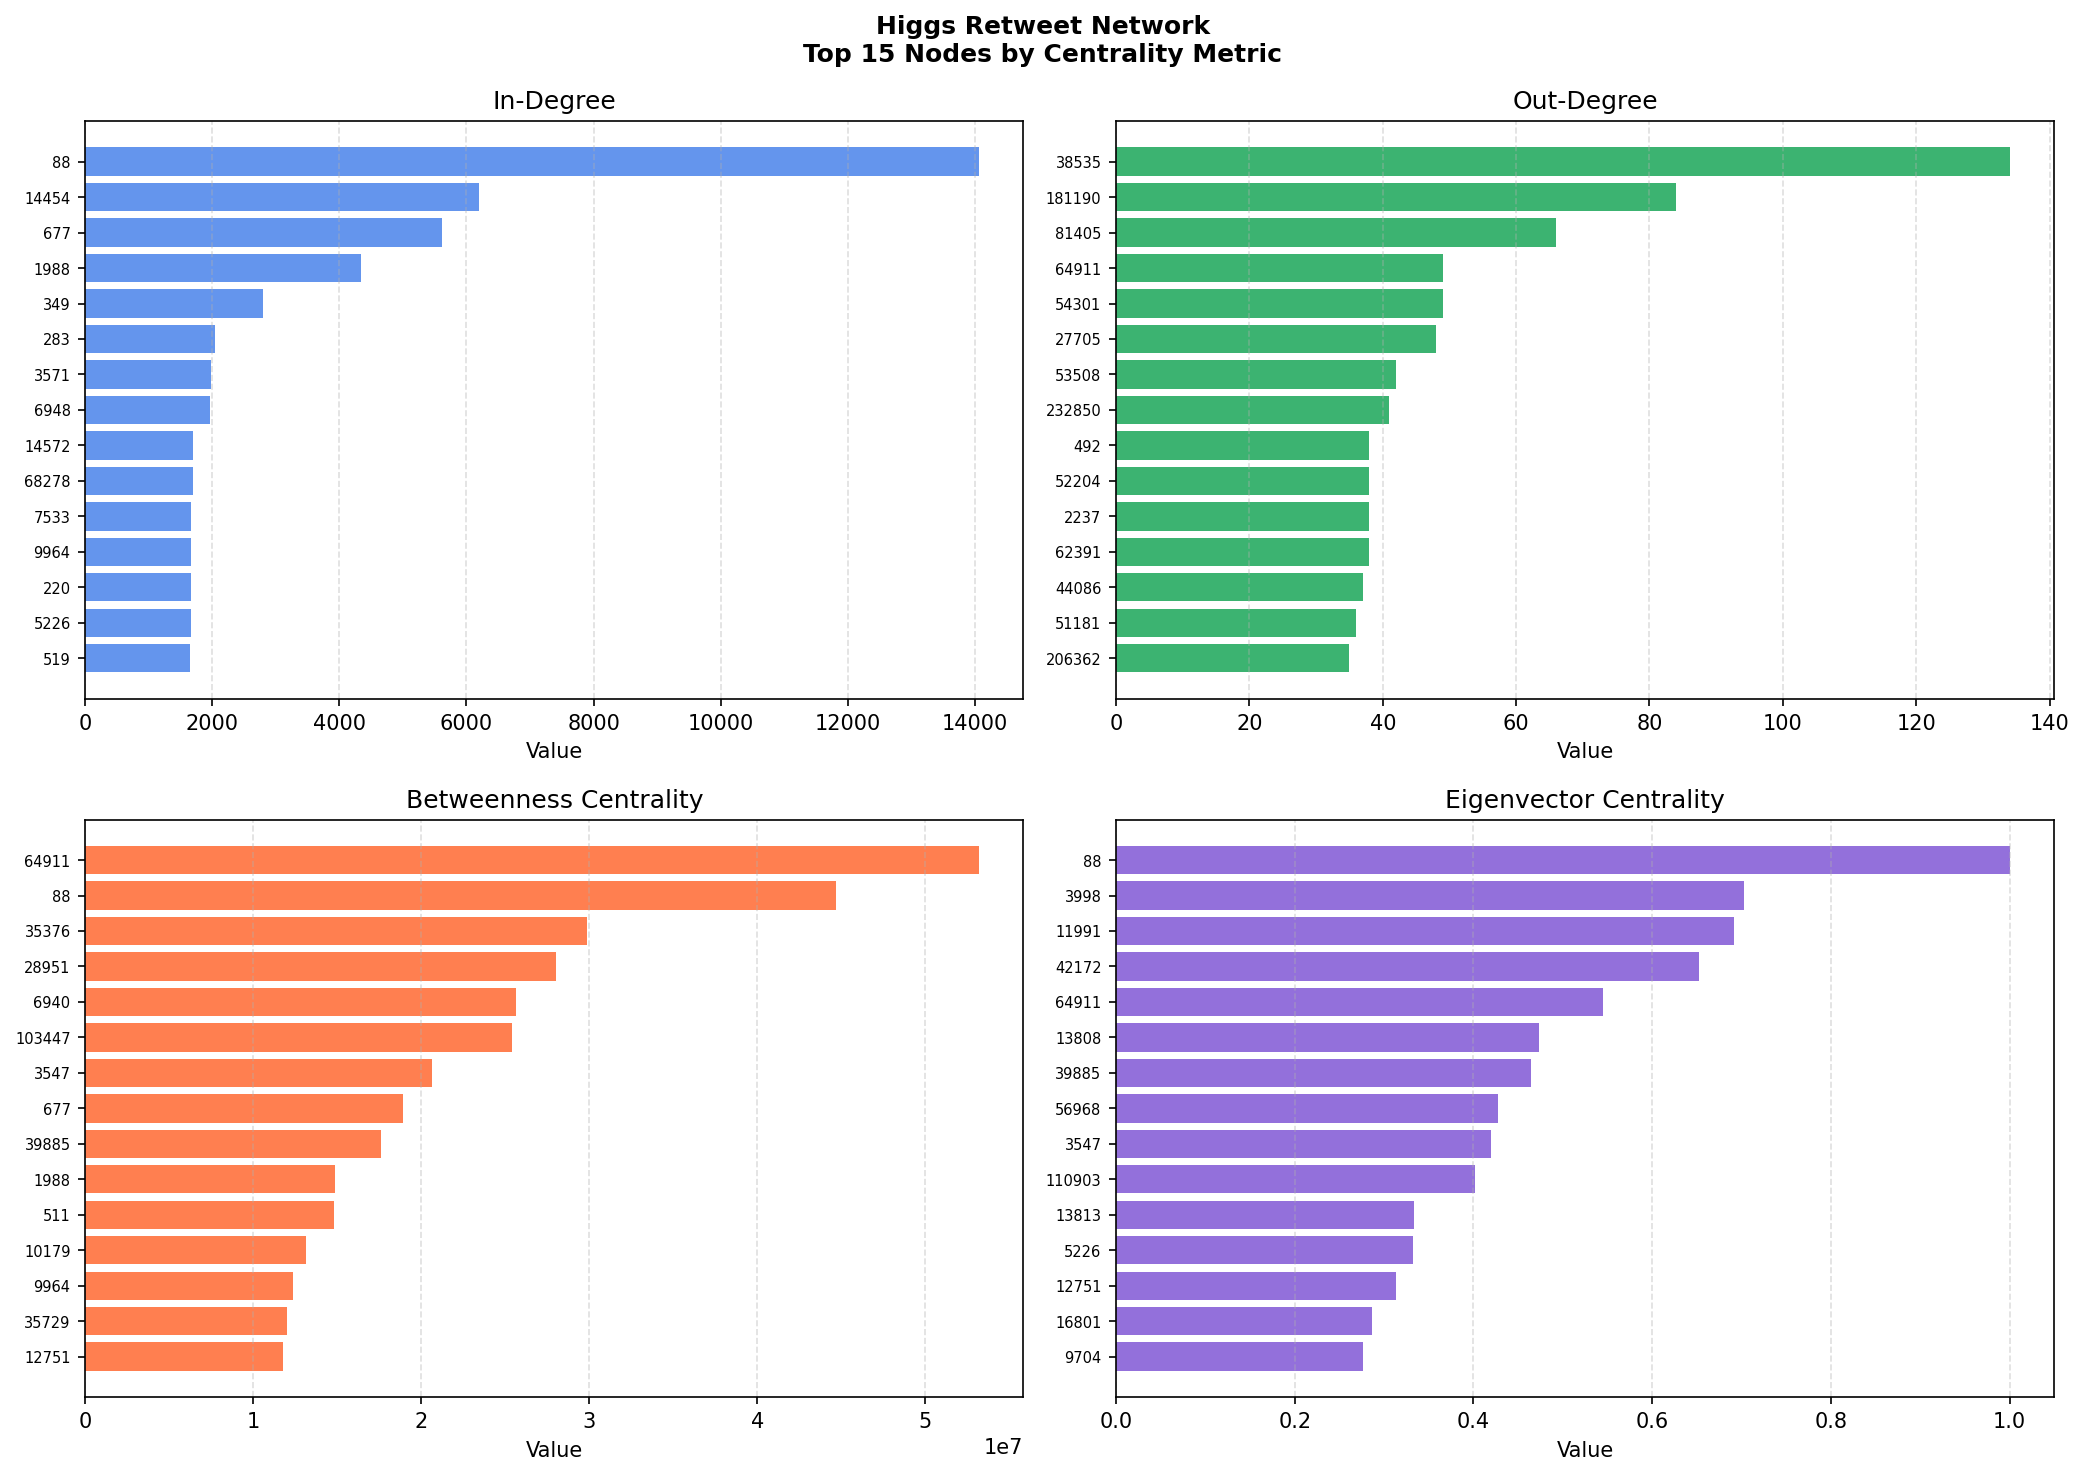
\includegraphics[width=0.95\linewidth]{figures/higgs_retweet_centrality.png}
    \caption{Top-15 nodes by each centrality metric in the Higgs Retweet network.
             Node \texttt{88} dominates in-degree (14{,}060 retweets) while
             \texttt{64911} leads in betweenness, confirming the hub--bridge
             distinction across all Higgs interaction types.}
    \label{fig:retweet_centrality}
\end{figure*}

\subsection{Top-10\% Metric Intersections}

Figure~\ref{fig:intersections} shows pairwise top-10\% intersections for
each network.
Several observations stand out:

\begin{itemize}
    \item \textbf{In-Deg $\cap$ Out-Deg} is the smallest intersection in all
          three networks, confirming that popular recipients generally do not
          also broadcast heavily — passive popularity and active participation
          are distinct roles.
    \item In the Retweet network, \textbf{Betweenness $\cap$ Eigenvector}
          yields 18{,}628 nodes — the largest pairwise intersection of any
          metric pair across all datasets — indicating that structural bridges
          and influential neighbors are strongly correlated in the retweet graph.
    \item The Reply network shows the tightest intersections overall,
          consistent with its smaller size and more conversational structure.
\end{itemize}

\begin{figure*}[ht]
    \centering
    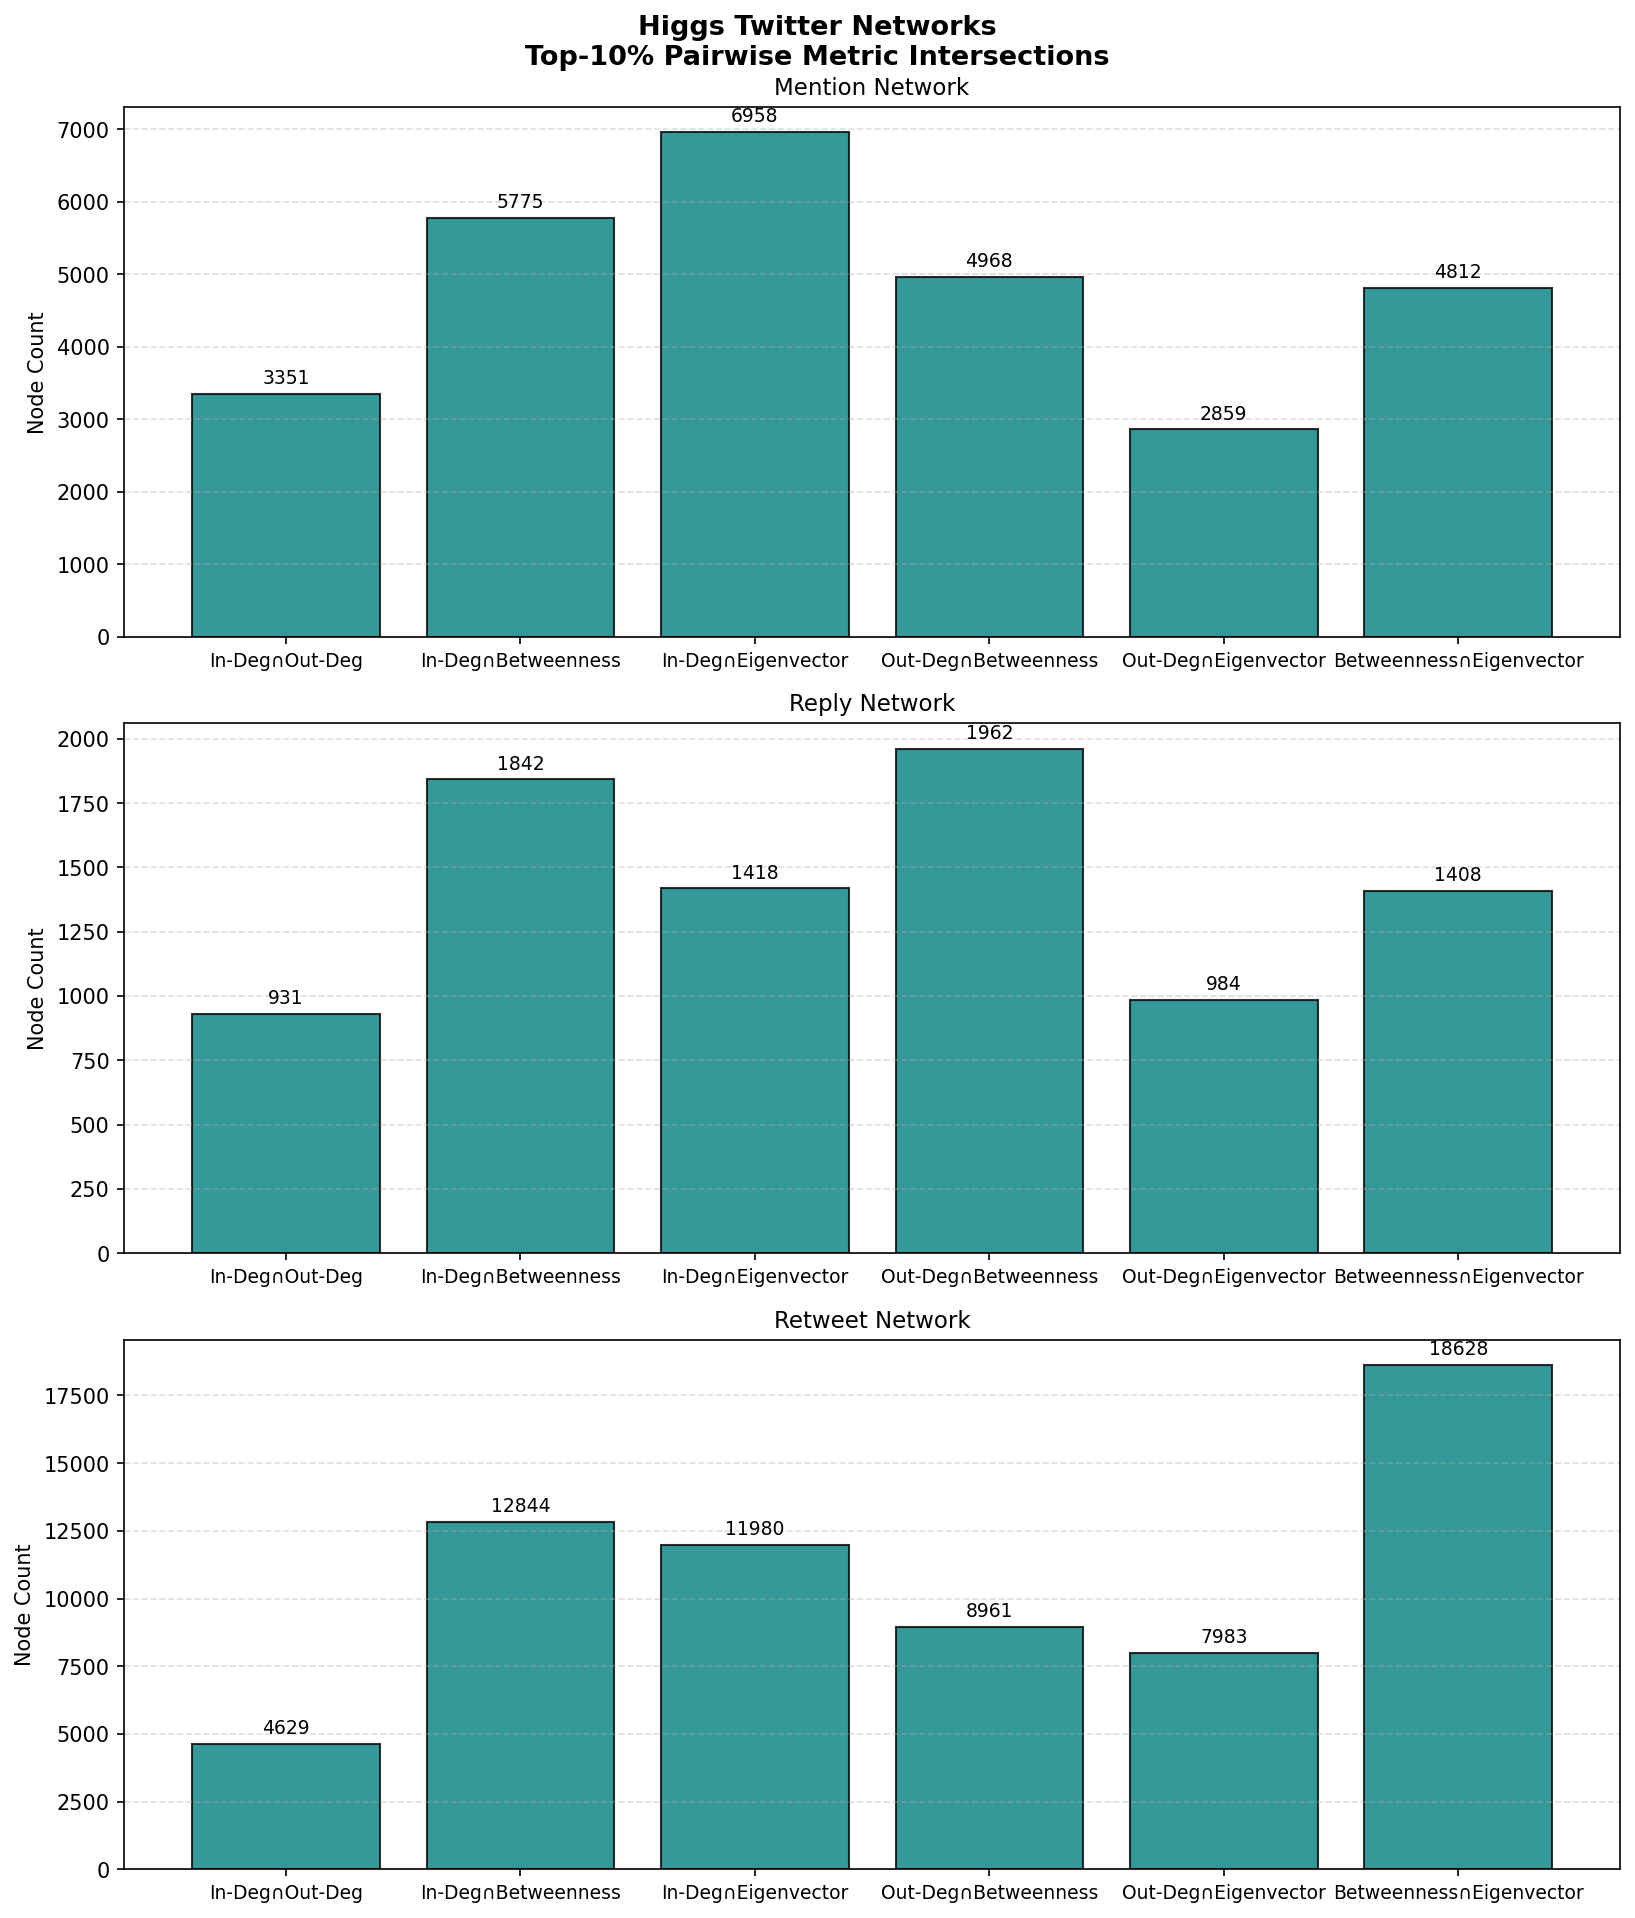
\includegraphics[width=0.78\linewidth]{figures/higgs_all_intersections.png}
    \caption{Top-10\% pairwise metric intersections for the Mention (top),
             Reply (middle), and Retweet (bottom) networks.
             In-Deg $\cap$ Out-Deg is consistently the smallest intersection,
             while Betweenness $\cap$ Eigenvector is the largest in the
             Retweet network.}
    \label{fig:intersections}
\end{figure*}

\subsection{Cross-Network Comparison}

Figure~\ref{fig:comparison} compares node count, edge count, and average
in-degree across the three Higgs networks.
The Retweet network is more than twice as large as the Mention network and
six times the size of the Reply network, reflecting the asymmetric
virality of the Higgs boson announcement.

\begin{figure*}[!t]
    \centering
    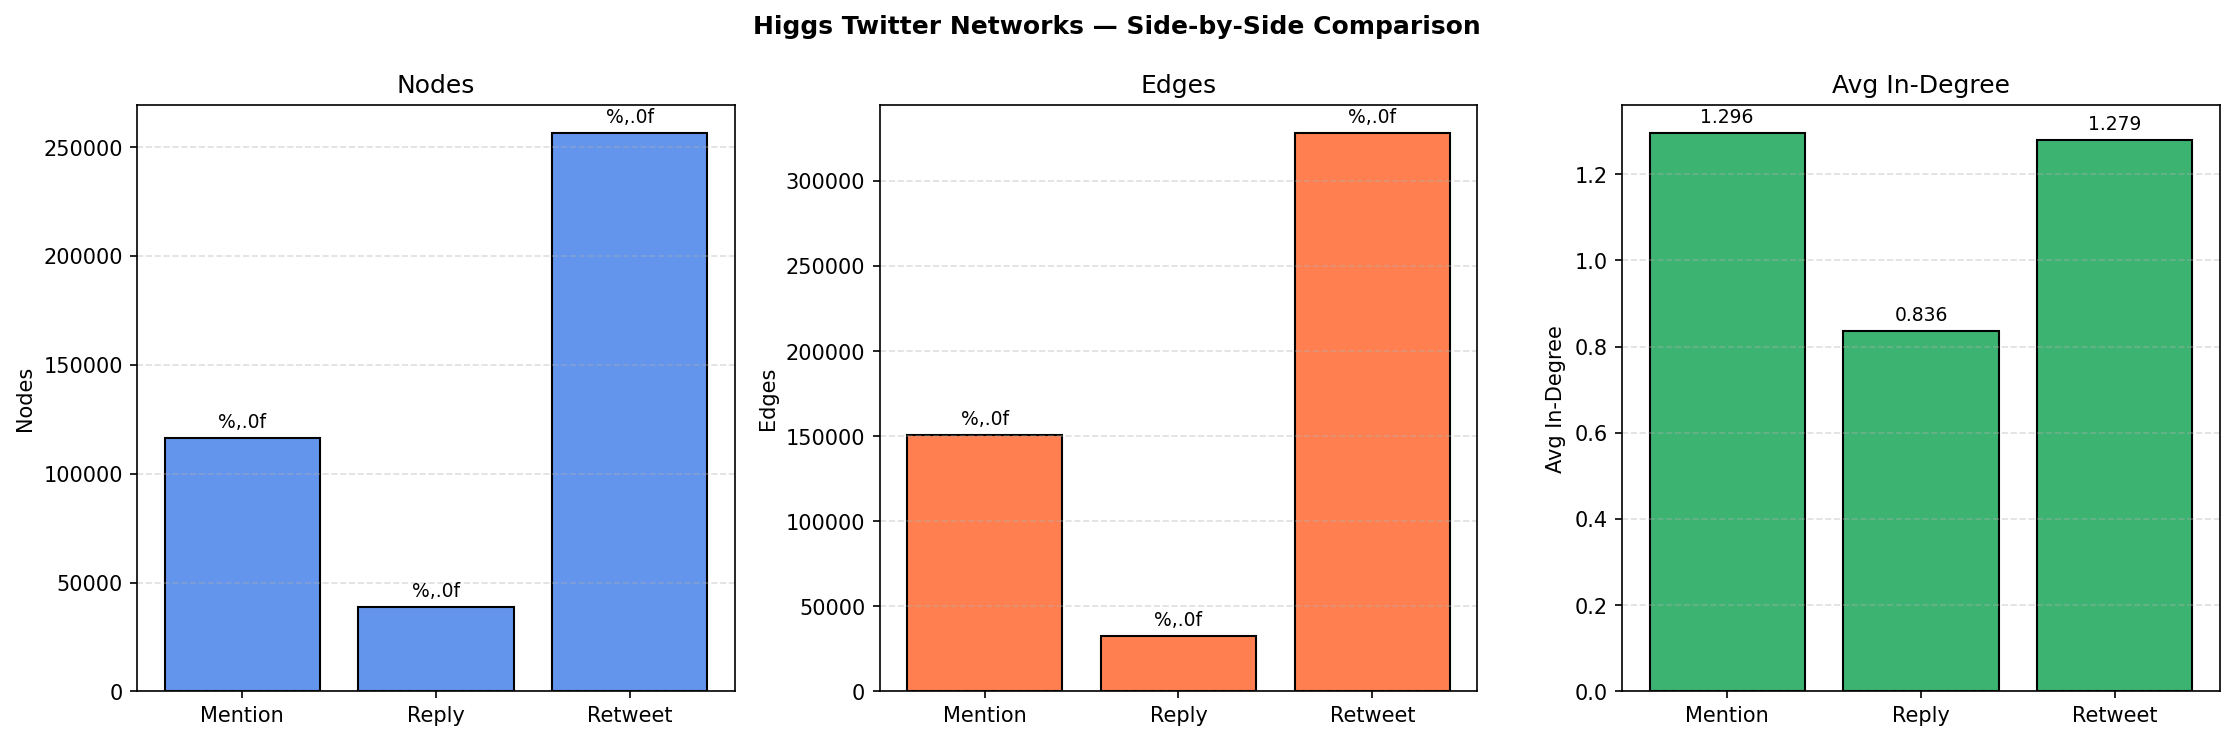
\includegraphics[width=0.48\linewidth]{figures/higgs_comparison.png}
    \hfill
    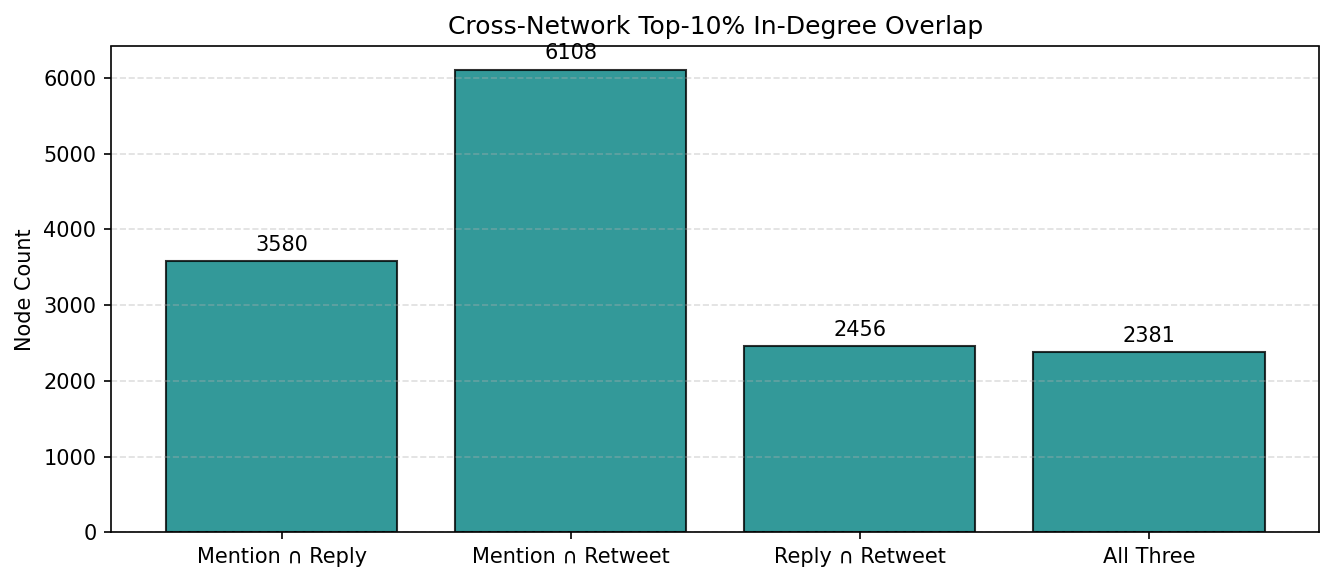
\includegraphics[width=0.48\linewidth]{figures/higgs_overlap.png}
    \caption{\textit{Left}: Side-by-side comparison of the three Higgs Twitter
             networks by number of nodes, edges, and average in-degree.
             \textit{Right}: Cross-network top-10\% in-degree overlap.
             Mention $\cap$ Retweet yields 6,100 shared high-influence users
             — the largest pairwise overlap — while only 2,301 nodes appear
             in the top 10\% across all three networks simultaneously.}
    \label{fig:comparison}
    \label{fig:overlap}
\end{figure*}

Figure~\ref{fig:comparison} (right) shows that 6,100 nodes appear in the
top 10\% by in-degree in both the Mention and Retweet networks — the largest
pairwise overlap — while only 2,301 nodes are consistently influential across
all three interaction types simultaneously.

\subsection{Enron Email Network}

Figure~\ref{fig:enron_centrality} shows the top-15 Enron nodes by each
centrality metric.
\texttt{sally.beck@enron.com} (COO) dominates both in-degree and betweenness,
indicating she was both a primary recipient and a critical communication bridge
across departments.
High out-degree belongs to \texttt{sally.beck} and \texttt{bob.ambrecht},
consistent with executive broadcast behaviour.
Notably, betweenness and eigenvector centrality surface different executives
than in-degree alone — \texttt{don.baughman} ranks highly in betweenness
despite modest in-degree, suggesting a broker role spanning otherwise
disconnected groups.

\begin{figure*}[ht]
    \centering
    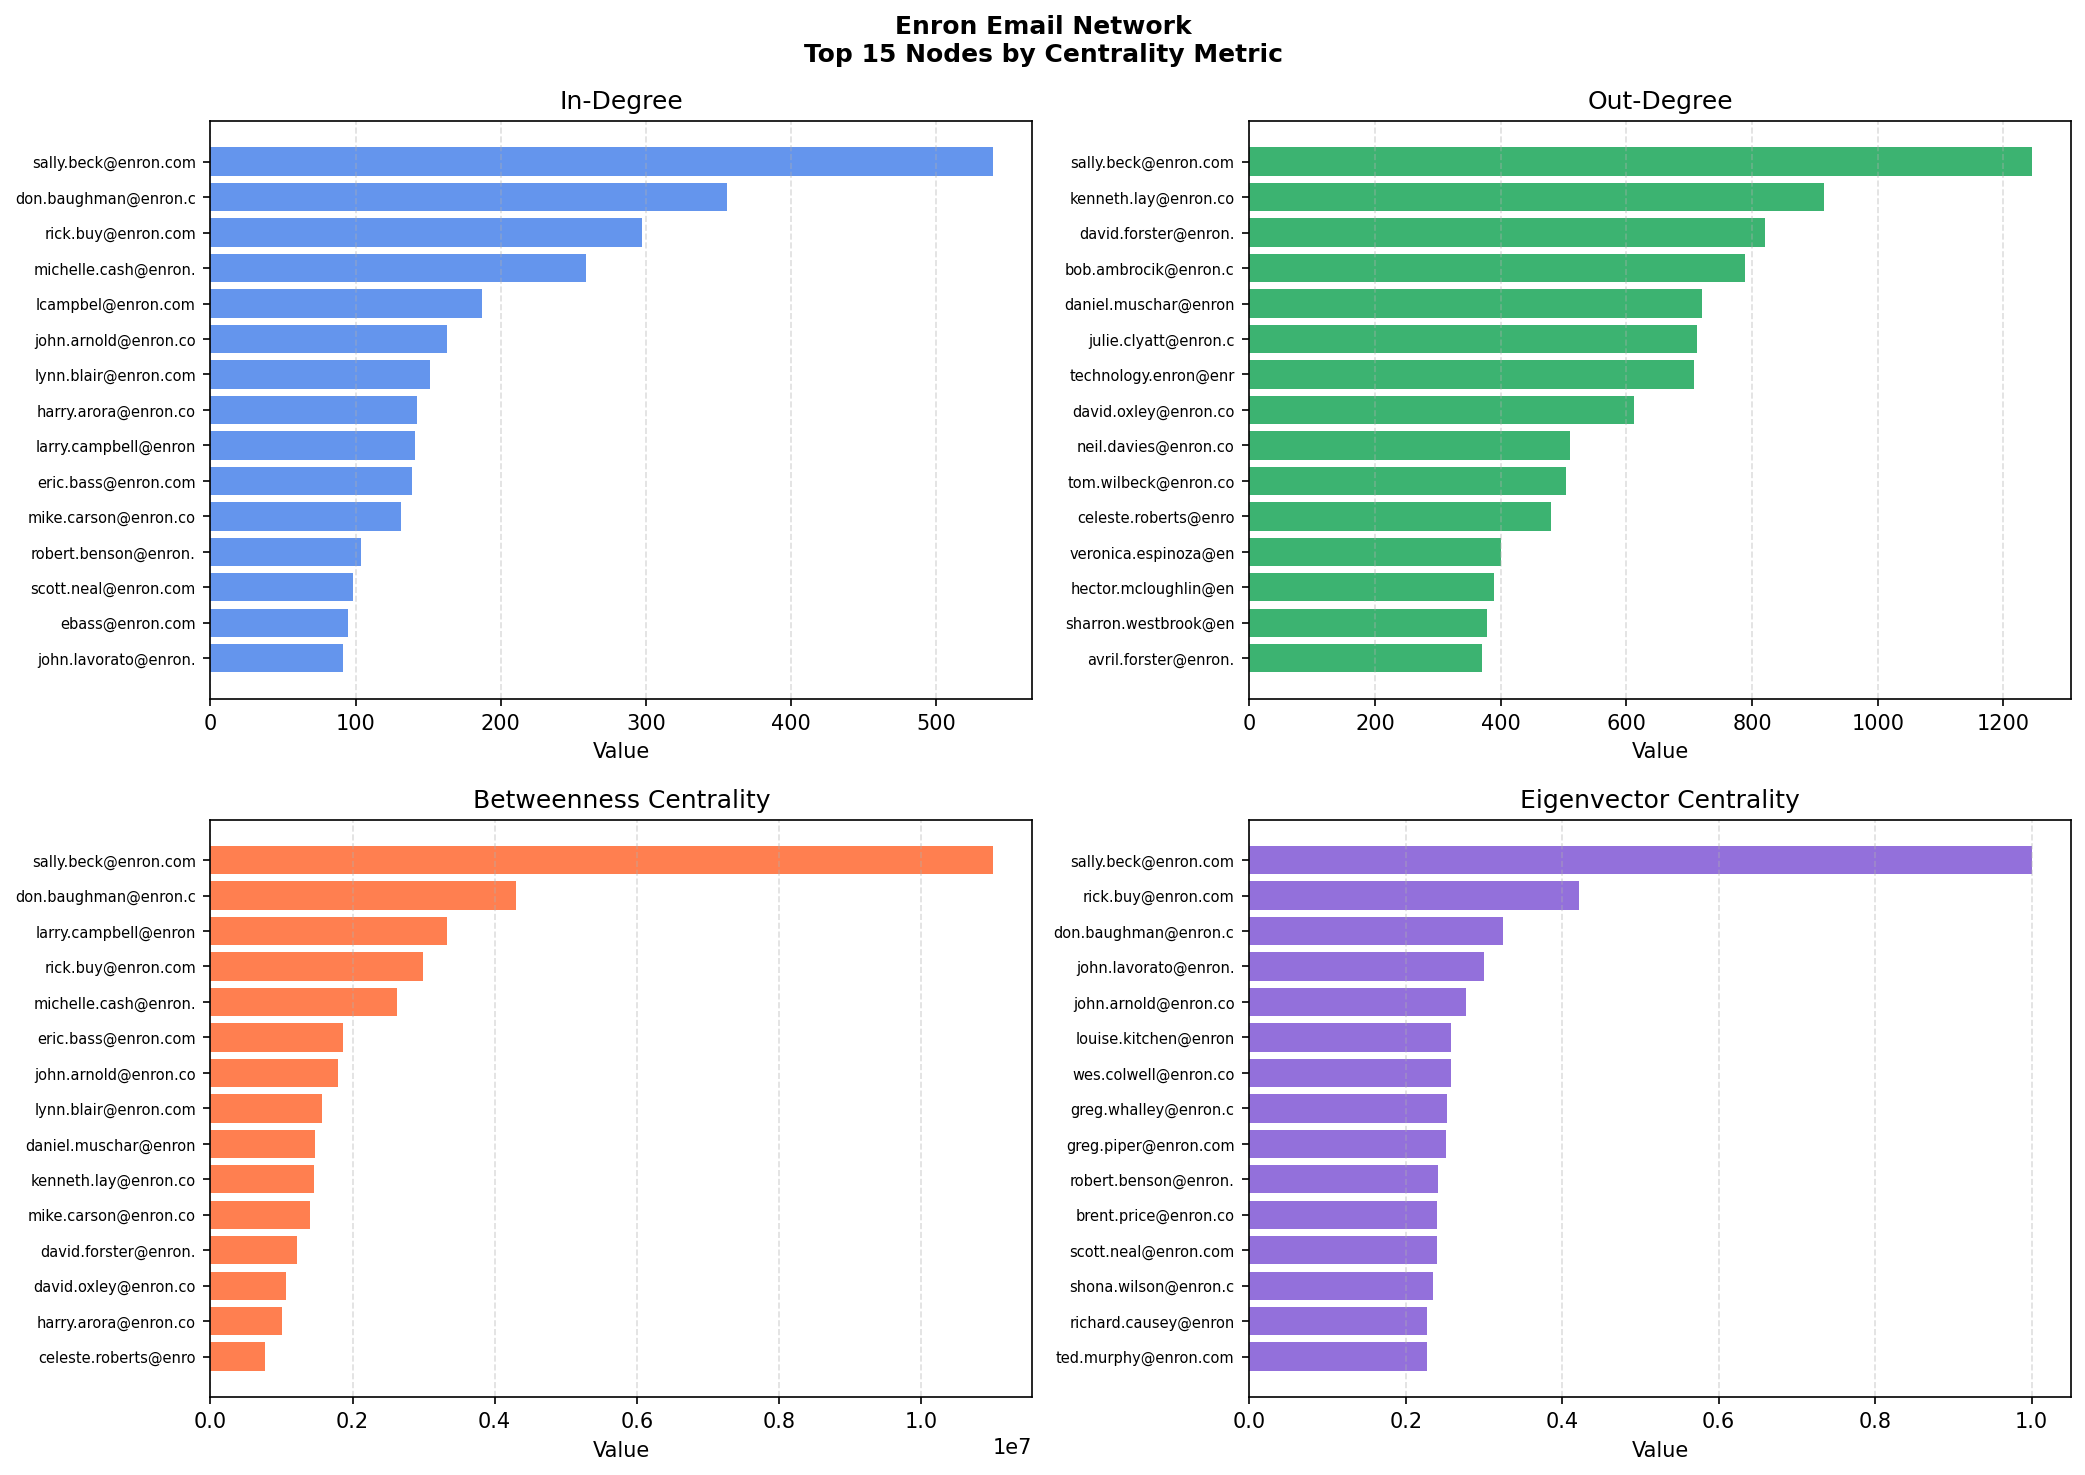
\includegraphics[width=0.95\linewidth]{figures/enron_centrality.png}
    \caption{Top-15 Enron email addresses by centrality metric.
             High in-degree nodes correspond to executive inboxes and
             distribution lists; high betweenness nodes represent
             organizational bridges between departments.}
    \label{fig:enron_centrality}
\end{figure*}

The Louvain algorithm identified 252
communities in the Enron network, as shown in Figure~\ref{fig:enron_comm}.
The distribution of community sizes is highly skewed, with a few large
communities (likely business units) and many small peripheral clusters.
Figure~\ref{fig:enron_exec} provides a richer view of the executive
sub-network, with node size proportional to degree and edge thickness
proportional to email volume.

\begin{figure*}[!t]
    \centering
    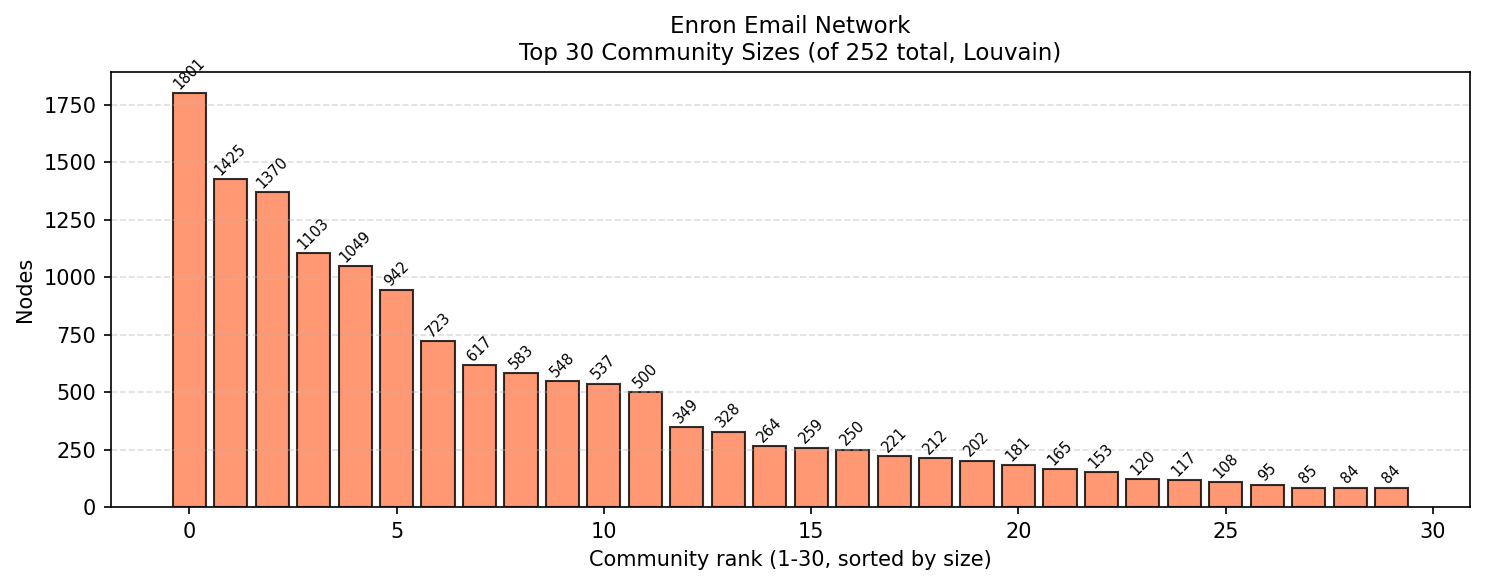
\includegraphics[width=0.55\linewidth]{figures/enron_communities.png}
    \vspace{0.5em}\\
    \includegraphics[width=0.95\linewidth]{figures/enron_exec_network.png}
    \caption{\textit{Top}: Louvain community sizes for the Enron email
             network (top 30 of 252 total), sorted by size. The rapid
             drop-off indicates a few dominant business-unit clusters and
             many small peripheral groups.
             \textit{Bottom}: Executive sub-network showing top senders
             for each VP/CEO. Node size is proportional to degree;
             edge thickness encodes email volume.
             \texttt{sally.beck@enron.com} (COO) is the largest hub.}
    \label{fig:enron_comm}
    \label{fig:enron_exec}
\end{figure*}

\subsection{Facebook Ego-Network}

Figure~\ref{fig:fb_deg} shows the degree distribution and Louvain community
structure of the Facebook network.
The 16 communities range from 19 to 548 nodes and likely correspond to the
distinct social circles of the ten anonymised ego users; the uneven size
distribution reflects the varying social reach of each ego.
In contrast to Enron's 252 fine-grained departmental clusters, Facebook yields
far fewer but larger communities, consistent with the tighter clustering and
higher average degree (21.8) of a friendship graph.

\begin{figure*}[!t]
    \centering
    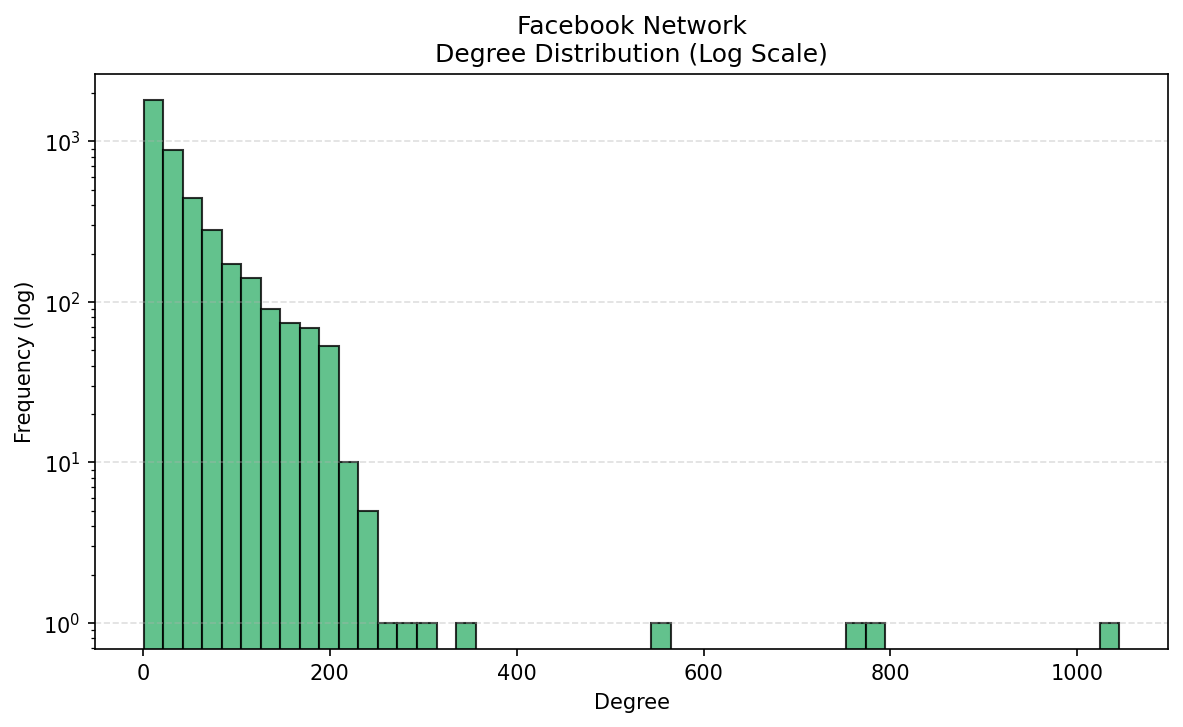
\includegraphics[width=0.48\linewidth]{figures/fb_deg.png}
    \hfill
    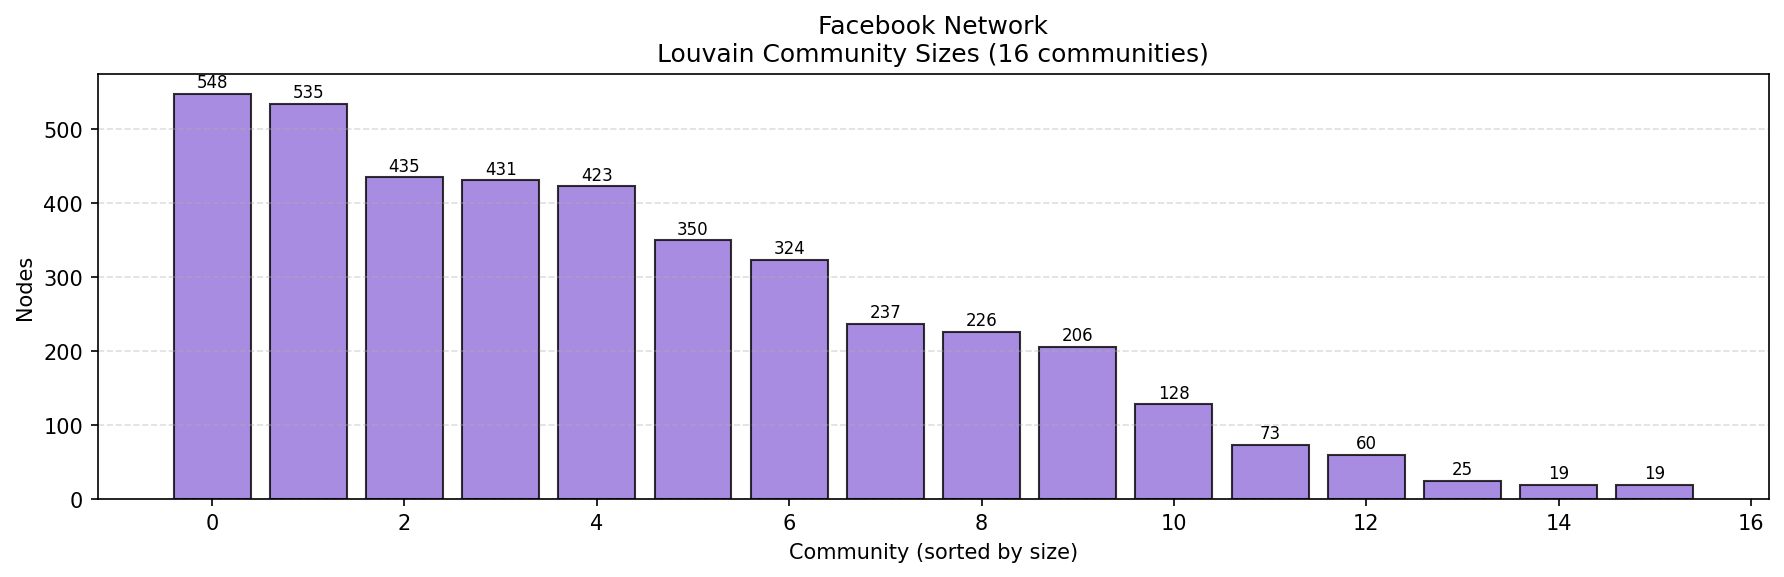
\includegraphics[width=0.48\linewidth]{figures/fb_communities.png}
    \caption{\textit{Left}: Degree distribution of the Facebook combined
             network (log scale). The distribution is heavy-tailed but
             less extreme than the directed Higgs networks, reflecting
             the reciprocal nature of friendship ties.
             \textit{Right}: Louvain community sizes for the Facebook
             network. The 16 communities range from 19 to 548 nodes and
             likely correspond to distinct social circles of the ego users.}
    \label{fig:fb_deg}
    \label{fig:fb_comm}
\end{figure}
